%TODO Hodai: get rid of the CPU (use processor/computational time...)
%TODO Hodai: find the correct word for "guarded automata"
%TODO Hodai: mybe add the symucopter project

\documentclass[11pt]{article}

\usepackage{graphicx}
\usepackage{tikz}
\usetikzlibrary{shapes.geometric, arrows, automata, positioning}
\tikzstyle{recNode} = [rectangle, minimum width=3cm, minimum height=1cm, text centered, rounded corners=0.1cm, draw=black]
\tikzstyle{recNodeB} = [recNode, draw=blue, fill=blue!10,text=blue!20!black]
\tikzstyle{recNodeG} = [recNode, draw=red, fill=red!10,text=red!10!black]
\tikzstyle{eNode} = [minimum height=1cm, text centered,text=blue!20!black]

\tikzstyle{arrow} = [thick,->,>=stealth,draw=black]
\tikzstyle{arrowB} = [thick,->,>=stealth,draw=blue]
\tikzstyle{arrowG} = [ultra thick,->,>=stealth,draw=red, dashed]

\newcommand{\comment}[1]{}

\newcommand{\uncomment}[1]{#1}


\usepackage{url}

\author{Hodai Goldman}
% (Hodaig@cs.bgu.ac.il) \\ \\Department of Computer Science, \\Ben-Gurion University of the Negev, Beer Sheva, Israel \\ \\Supervisor: Dr. Gera Weiss}
\date{\today}
\title{\LARGE {\bf Computational resource management of multi channel controller}}

\usepackage{hyperref} % makes table of contents links
\hypersetup{
    colorlinks=true, %set true if you want colored links
    linktoc=all,     %set to all if you want both sections and subsections linked
    %linkcolor=blue,  %choose some color if you want links to stand out
    %citecolor=black,
}

\begin{document}
\begin{titlepage}
\maketitle
\end{titlepage}

\tableofcontents

\section{Introduction}
\subsection{motivation and overview}
\label{sec:Background}
Today's computer power allows for consolidation of controllers towards systems where a single computer regulates many control loops, each with its varying needs of computation resources.
This brings two research challenges that we intend to attack in this thesis:
\begin{itemize}
	\item How to schedule control tasks in order to achieve good performance in terms of control measures (overshoot, convergence time, etc.), within the still limited computation resources?
	\item What is a good interface for co-design of scheduling and control?
\end{itemize}

%TODO - I think the next paragraph is too much digging
While it is possible to build control systems using standard operating systems, either real-time or desktop, with static or with dynamic scheduling schemes, there is an agreed opinion in the control community that these do not serve well for the purpose outlined above. For example, in~\cite{Cervin}, the authors say: 
\begin{quotation}
`The delay and jitter introduced by the computer system can lead to significant performance degradation. To achieve good performance in systems with limited computer resources, the constraints of the implementation platform must be taken into account at design time.'
\end{quotation}
Similar views are expressed also in other papers~\cite{RTComposer,Shlomo,UPenn-Pant}.
 
Desktop type operating systems, like Windows and Linux, schedule for computational efficiency but do not allow for worst-case performance guarantees. Real-time operating systems, on the other hand, sacrifice some efficiency for timing predictability, but the type of timing guarantees that such systems provide usually are not directly guaranteeing the control performance of the system. 
When using such operating systems for control, engineers usually apply controllers that work in a fixed periodic manner witch the control behavior becomes deterministic and control performance can be guaranteed. This is not efficient because resources can be better utilized if controllers act at higher frequencies only when needed.

In this work we show how to combine the efficiency of dynamic scheduling with the predictability of real-time scheduling, in a way that is more suitable for control systems then periods and deadlines.
We show that applying control computations at dynamically adjustable periodic, and with variable computational demands, based on real-time information, allows for better utilization of the computational resources and therefor better control performance.

The main innovation of this work is the system architecture design.
In practice most of the real-time control systems designs consists of to separated elements, (1) control and estimations tasks, and (2) a task scheduler which divide the resources (CPU time) between all tasks. 
Although those two parts are constantly affected by each other they barely communicate, this lead to static (constant) scheduling regardless of the current state or needs of the system.
In this thesis we develop an architecture design for control systems in witch the scheduler (2) is aware of the current state of the system, and makes \textit{state depended} scheduling for that state. 
We show how allocate resources by \textbf{current} needs give better resoults than allocate resources for the \textbf{worst-case} needs.

 
\section{Problem Statement}
\label{sec:Problem}
We are concentrate on close feedback control loop based systems as shown in Figure~\ref{fig:control loop}. 
We assume a close feedback control loop where the physical plant, \textit{System} state ($x$), is monitored via an array of sensors (\textit{Sensing}) which produce raw data ($y$) that represents noisy sample of some functions of the state variables. 
We assume uncertainty observations from the sensors so, after sensing, an entity called \textit{State Estimator} aggregates the raw data from all the sensors and makes an educated estimation ($\hat{x}$) of the current state. Then the \textit{Control Law} entity generates the controller outputs ($u$), control the actuators, to change the state of the system in order close the gap between the current estimated state and the reference desire state (\textit{Input} $r$).

The current state-of-the-art computer embedded control systems, as descibed e.g. in~\cite{Celvin}, are developed as follows, control engineers first design control tasks (control and estimation tasks) as periodic computations, then they specify the required periodic frequency for the task, and then software engineers design a scheduler that ensures the periodic frequency requirements are met. 
The last step is usually done using pre-computed knowledge of the expected (maximum) duration of the tasks.
Note that in order to ensure that the controlled plant is always properly maintained, for example engine temperature never exceeds maximal safe temperature, the periodic frequency must be tuned for the worst-case state that the system might be in.

We show how to achieve better performance and better resource utilization for control systems by using richer and more flexible requirements model for the tasks.
Specifically, we develop tools and methodologies such that control engineers are able to specify more accurately the requirement features of their control tasks, that the scheduler will use for executing dynamic resource assignment that will, at the same time, guarantee required control performance and will be efficient in its use of computational resources. 

\begin{figure}[]
    \centering
    
    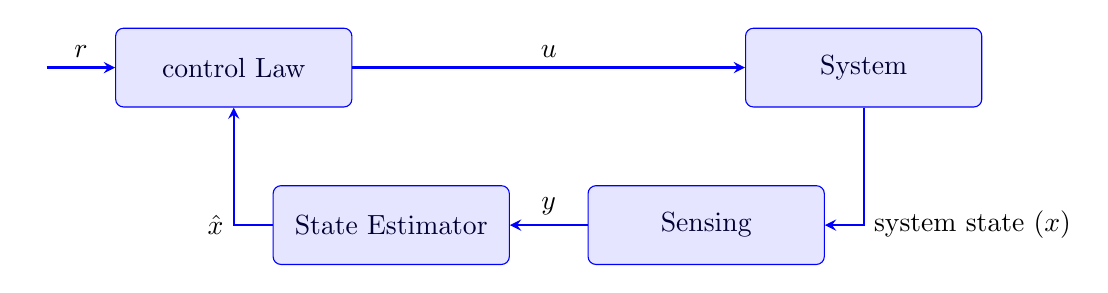
\begin{tikzpicture}[node distance=2cm]
        \node (in) [eNode] {};
        \node (control) [recNodeB, right of=in, xshift=0.5cm] {control Law};
        \node (sys) [recNodeB, right of=control, xshift=6cm] {System};
        \node (sensor) [recNodeB, below of=sys, xshift=-2cm] {Sensing};
        \node (estimator) [recNodeB, below of=control, xshift=2cm] {State Estimator};
        
        \draw [arrowB] (in) -- node[above] { $r$} (control);
        \draw [arrowB] (control) -- node[above] { $u$} (sys);
        \draw [arrowB] (sys) |- node[right] { system state ($x$)} (sensor);
        \draw [arrowB] (sensor) -- node[above] { $y$} (estimator);
        \draw [arrowB] (estimator) -| node[left] { $\hat{x}$} (control);
    \end{tikzpicture}
    
    \caption{A typical close feedback control loop where the physical plant (\textit{System}) is monitored via an array of sensors (\textit{Sensing}) which produce noisy sample of the state variables $y$. 
    And after sensing, \textit{State Estimator} aggregates the raw data from all the sensors and produce estimation of the current state $\hat{x}$. Then the \textit{Control Law} produce output to the actuators ($u$) in order to close the gap between the current estimated state and the reference state ($r$).
    \label{fig:control loop}}
\end{figure}



\section{Architecture: Automata Base Scheduler}

\begin{figure}[]
    \centering
    
    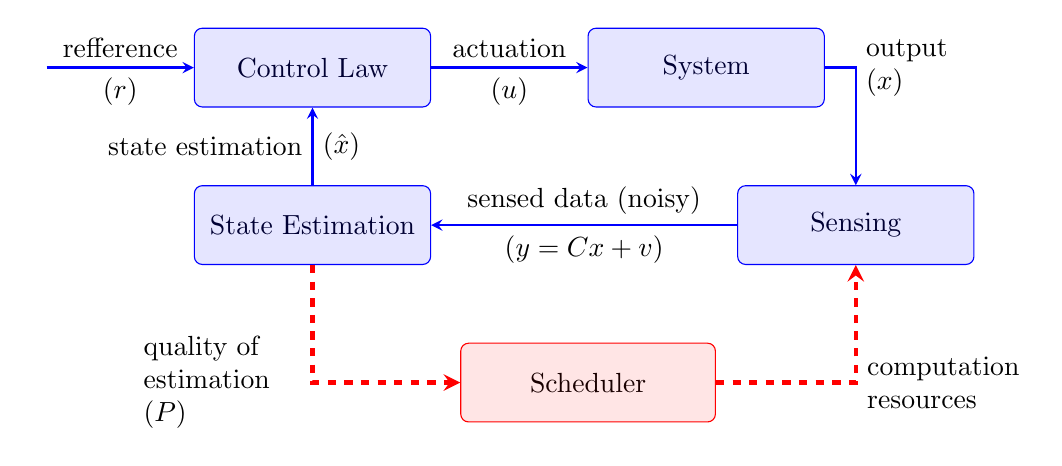
\begin{tikzpicture}[node distance=2cm]
    \node (in) [eNode] {};
    \node (control) [recNodeB, right of=in, xshift=1.5cm] {Control Law};
    \node (sys) [recNodeB, right of=control, xshift=3cm] {System};
    \node (sensor) [recNodeB, below of=sys, xshift=1.9cm] {Sensing};
    \node (estimator) [recNodeB, below of=control] {State Estimation};
    \node (sched) [recNodeG, below of=estimator, xshift=3.5cm, text width=3cm] {Scheduler};
    
    \draw [arrowB] (in) -- node[above] {refference} node[below] {($r$)} (control);
    \draw [arrowB] (control) -- node[above] {actuation} node[below] {($u$)} (sys);
    \draw [arrowB] (sys) -| node[right,text width=1cm] {output ($x$)} (sensor);
    \draw [arrowB] (sensor) -- node[above] {sensed data (noisy)} node[below] {$(y = Cx +v$)} (estimator);
    \draw [arrowB] (estimator) -- node[left] {state estimation} node[right] {($\hat{x}$)} (control);
    
    \draw [arrowG] (sched) -| node[right,text width=2cm] {computation resources} (sensor);
    %\draw [arrowG] (sched) --  node[right] {$var(v)$} (estimator);
    \draw [arrowG] (estimator) |- node[left,text width=2cm] {quality of estimation ($P$)} (sched);
    
    
    \end{tikzpicture}
    
    \caption{A general scheduling framework. Each control loop (depicted in blue) informs the resource allocator (Scheduler) of its quality of estimation and the allocator allocates accordingly the computation resources among all the control loops, in order to maintain valid estimation quality. 
    %The underlying assumption here is that the noise in the sensed data is a function of the amount of computation resources. We assume that the more resources are invested in sensing the better (less noisy) sensed data is obtained.
        \label{fig:general_hybrid_loop}}
\end{figure}

\begin{figure}[h]
    \centering
    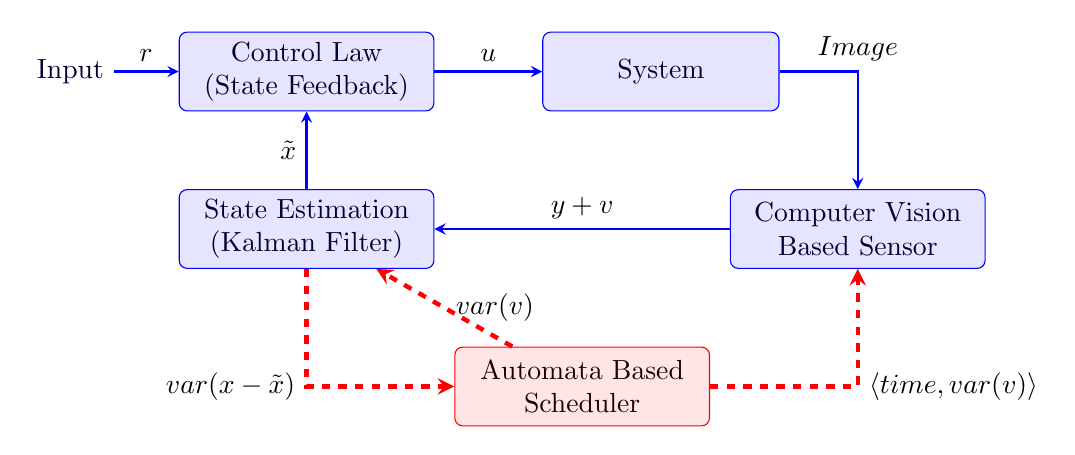
\begin{tikzpicture}[node distance=2cm]
    \node (in) [eNode] {Input};
    \node (control) [recNodeB, right of=in, xshift=1cm, text width=3cm] 
    {Control Law (State Feedback)};
    \node (sys) [recNodeB, right of=control, xshift=2.5cm] {System};
    \node (sensor) [recNodeB, below of=sys, xshift=2.5cm, text width=3cm] 
    {Computer Vision Based Sensor};
    \node (estimator) [recNodeB, below of=control, text width=3cm] 
    {State Estimation (Kalman Filter)};
    \node (sched) [recNodeG, below of=estimator, xshift=3.5cm, text width=3cm] {Automata Based Scheduler};
    
    \draw [arrowB] (in) -- node[above] {$r$} (control);
    \draw [arrowB] (control) -- node[above] {$u$} (sys);
    \draw [arrowB] (sys) -| node[above] {$Image$} (sensor);
    \draw [arrowB] (sensor) -- node[above] {$y+v$} (estimator);
    \draw [arrowB] (estimator) -- node[left] {$\tilde{x}$} (control);
    
    \draw [arrowG] (sched) -| node[right] {$\langle time,var(v) \rangle$} (sensor);
    \draw [arrowG] (sched) --  node[right] {$var(v)$} (estimator);
    \draw [arrowG] (estimator) |- node[left] {$var(x-\tilde{x})$} (sched);
    
    \end{tikzpicture}
    
    \caption{The controller framework we will implement, the \textit{scheduler} will allocate CPU time ($\langle time,var(v) \rangle$) for the \textit{Computer Vision} task base on the state estimation certainty using guarded Automata.
        \label{fig:hybrid_loop}}
\end{figure}

As describe in Section~\ref{sec:Problem} control systems have two main parts: \textit{state estimation} and \textit{controller}. 
All the common used techniques for controllers, e.g PID, are relatively low resources consumers and there is no real justification of optimizing it, but this is not always the case for estimation process, some times there are heavy computational tasks as part of state estimation task, this refers to both the estimator and sensing stage.
The sensor can be complex computations of Global Positioning System (GPS) in small processor or even camera with heavy computer vision.
% TODO
Those sensing task need to run in real-time and can interfere with rest of the system tasks.
In out architecture we concentrate more in those heavy sensing processes in order to improve the resource utilization and control performance.
%One wide used example is the use of computer vision in UAV's 
(See~\ref{state estimation & why choose the window mission})

%TODO - i think fig:general_hybrid_loop is Unnecessary and fig:hybrid_loop is enough 
The architecture of control system as we believe, is illustrated in Figure~\ref{fig:general_hybrid_loop}.
The architecture, that is based on modern controller architecture where the system has multiple controlling tasks, comes to support an efficient scheduling protocols in modern control systems consisting of a processor that runs all the tasks of many independent control loops in the system. 
The current state of art, as described above and as we observed, e.g. in the code of APM~\cite{APM}, is that the designers of each task, control or estimation task, specify a fixed rate for invocations of the corresponding task (called \textit{period}).
% TODO: Use the terminology of the figure
In our methodology, there is a richer and more intense interaction between the \textit{Scheduler} and the control loops. Each control loop (blue components in the Figure~\ref{fig:general_hybrid_loop}) will tell the \textit{scheduler} of its level of certainty ($P = var(\hat{x} - x)$) and the allocator will allocate resource (processor time) based on this data, meaning the \textit{scheduler} allocate resource dynamically based on the system current needs rather than the worst case needs.
%TODO - ?? what next centence mean? needed?
%TODO: This can be useful on its own sake or together with a mathematical analysis that allows to use this feedback mechanism to certify some pre-defined specifications of state certainty or stability is maintained.

%TODO - probably need to be in the Tests section
Our methodology is general and may be applicable in a wide range of applications. However, in this initial phase of the research, we focus on a specific sub-domain and in handling all technical issues in order to prove the concept.
In this thesis we develop and implement a vision based controller for drone (see Section~\ref{sec:tests}) and analyze the concept with it.

%TODO - probably need to be in the Tests section
TODO - need to fix here!!!
\comment{
As shown in Figure~\ref{fig:hybrid_loop}, the system framework consists of an interaction between the scheduler and the control loops, in this case the estimator (\textit{State~Estimator}) accuracy strongly depends on the sensing task (\textit{Computer~Vision}) and they both collaborate with the \textit{scheduler} in order to achieve their \textbf{control objectives} (g.e. stability).
In this framework the scheduler is part of the control logic and therefore it can make scheduling decisions based on the current control state, the scheduling of \textit{Computer~Vision} task depends on the accuracy of state estimation.
For example, if the vision is clear, the \textit{Computer~Vision} will produce good measurement of the \textit{System} and therefore good accuracy will be achieved so the \textit{Scheduler} can allocate less computation time to the heavy \textit{Computer~Vision} task and still remain stable while allocating more CPU to others control loops or to background tasks (like navigation).

We will use an existing open-source implementation of drone software as a basis for our experimentation. However, the above collaboration requires to re-adjust some parts of the control system, e.g. the \textit{State~Estimator} needs to work with variable error variance of \textit{Computer~Vision} measurement,  the \textit{Computer~Vision} needs to be able run within variable time limits, and the tasks pre-defined requirements need to be re-adjusted in order to define the relation between tasks such as \textit{Computer~Vision} and \textit{State~Estimator}.
}

% TODO - make some connection
Below we will dive in each part of the new architecture and explain how it should be adjusted.

\subsection{Sensors}
\label{sec:sensors}
The sensing process are assumed to be periodic task. 
In order to allow dynamic scheduling it must be able to execute in a variable period between executions or to allow control of the execution duration time.
There are two general approaches we consider for this task: use \textit{any-time} algorithms or finite \textit{execution-modes} based tasks.
\textit{any-time} algorithms are algorithms that always try to improve the solution quality, for sensing processes, we can define deadline for the ``searching" process every execution, ??? present any-time solution for image processing~\cite{Shlomo}.
%TODO - "its also can be apllyed to general task by avaraging berst of exeqution in short time
%TODO also used by "anytime"
%TODO contract-based
Set of \textit{execution-modes} based, a discrete version influence from ``contract-based'' presented by ??? Pant~\cite{UPenn-Pant}, here each sensing task have finite number of ``operation modes'', e.g. different algorithms to proximate the same observations value, then the scheduler can perform the apropriate mode for every cycle.

For simplicity, we only work with \textit{execution-modes} based sensing tasks, all the modes are pre-defined and identified by a pair $\langle Duration, Variance \rangle$,
which define the error $Variance$ of this mode and the run-time $Duration$ is the of this mode. 
We assume that longer modes produce solution with smaller error variance.
%TODO - reed a litle the article (\cite{UPenn-Pant}) and re-write the next.
%TODO - check if Anitime reserch (\cite{Shlomo}) can fit here.
%TODO - Make sure that we use the terms contract-base and any-time correctly

\subsection{State Estimator}
\label{sec:estimator}
% kalman filter & ...
% seperation rule of kalman

State Estimator (the filter) is part of the estimation process, this unit receive the measurements ($y$) from the \textit{Sensors} and produce from them the state estimation required by the controller ($\hat{x}$).
When the \textit{Sensors} is accurate enough we may be able to pass it directly to the \textit{Controll Law} ($\hat{x} = y$), but usually the measurement is noisy and the main goal of the State Estimator is to reduce this noise from the measurement (see Section~\ref{sec:kalman}).
%TODO mybe add this: some times the sensor measure not mesure the needed state parameters, for example if we need to know the amount of water in the botle baut we only know the flow during all the rime we need to integrate in order to know the quantity.

If one consider using the optimal estimator Kalman filter (describe at Section~\ref{sec:kalman}) in the estimation process, one of the parameter that need to be consider in calculation is the covariance of sensor error (noted by $R$ in Section~\ref{sec:kalman}).
But in the new framework the sensor have diferents operation modes with variable error covariance, this means that we need to have also variable state estimators correspondingly.
In order to adjust the sensor error covariance, each cycle the scheduler will inform the state estimator about the new error covariance, and the state estimator will use corresponding parameters to make the next estimation.
%TODO - if the next is included need to read and learn "time-variant kalman filter"
%The second parameter that may be problematic is the state evolution in time ($A$ matrix in KF), which is defined for specific time period, and need to be adjusted if we use variable period, or maybe use time-variant kalman filter.

\subsection{Control Tasks} 
\label{sec:control} 
The control task (regulator) itself (\textit{Control Law} in Figure~\ref{fig:general_hybrid_loop}) is responsible for closing the gap between current state estimation ($\hat{x}$) and the reference state ($r$), by manipulating the system actuators (e.g. changing the speed of the motors), that output to the actuators is noted by $u$.

%Optimal estimation or optimal control law is not guarantee the overall optimal feedback controller, but as Kalman prove, 
The control task is usually a very low CPU consumer and been well studied~\cite{Bennett,Cervin}. Hence, the control task is not needed to be manipulated.
For our testing we use the commonly used and well known technique from control theory called PID, A proportional-integral-derivative controller.
In this technique the control output is based on the physical knowledge of the system dynamics, and have three variable parameters (P, I and D) that define the controller convergence behavior \cite{PID} ???.

%TODO
\comment{
We also plan to try to use an ``adjustable'' LQR (Linear-quadratic regulator) control, as follows.
LQR is an optimal controller that take into account the level of certainty of the state estimation. 
Is usually a hard task to know the certainty of estimation, but in our case we need to calculate it anyway, and we mark it as $var(x-\tilde{x})$.
We will make LQR ``adjustable'' in the sense that each iteration the controller will consider the new (variable) $var(x-\tilde{x})$. This is similar to the architecture we proposed for the estimator.
We will check if adjustable LQR has significant advantages over PID in cases were we have variable certainty of estimation.
}

\subsection{Computation Resource Scheduler: Automata Based Scheduler}
\label{sec:scheduler}

Real-time systems are mostly composed of multiple real-time tasks, tasks with time constraint, for example task that must response to an event within specified time constraints.
The purpose of schedulers in such systems is to allocate the limited computational resources (CPU time) within all the task in the system. To do so, we need a well defined interface between the real-time tasks and the scheduler.

The most common way of describing the requirements of a real-time component is to specify a period, sometimes along with a deadline, which gives the frequency at which the component must execute. 
The designer of the component makes sure that the performance objectives are met as long as the component is executed consistent with its period. The scheduler guarantees that all components get enough resources.
%not directly in this article
Specifying resource requirements using periods has advantages due to simplicity and analyzability, but has limited expressiveness, as elaborated in~\cite{RTComposer}. 
%For example, a specification such as “execute the component every 5ms” does not say whether the scheduler should or should not execute it more frequently if enough computing resources are available, and if a component has multiple methods, say, for different control tasks, each needing a different period, the requirement cannot be naturally captured by a single period.





% TODO - stop here!
\subsubsection{The Proposed Scheduling Methodology}
In this thesis we develop a new methodology for allocation resources. We focus on how should engineers describe the requirements of a real-time component.
To simplify, we will assume that the resource is allocated in discrete \textit{time slots} of fixed duration in the style of time-triggered architecture~\cite{RTComposer}.
%TODO - read again this section
%We will develop automata based (hybrid automata) methodologies and schedulers based on the work of Alur~\cite{RTComposer} and Bukra~\cite{Merav}, and will demonstrate with measurable data how they improve the performance of real flying drones (see Section~\ref{sec:results}).
The specification framework for resource requirements is based on \textit{Nondeterministic $\omega$-automata} (finite automata over infinite words)~\cite{???}.
Automata can be more expressive for describing specific requirements, and they are composable, i.e., it is easy to compose all the tasks requirements into an integrated automata, and its easy to analyze and manipulate using tools like GOAL~\cite{???}.


%TODO - what we do with $Acc$
Formally \textit{task specification automata} is defined, similarly to Nondeterministic $\omega$-automata, as tuple $A=(Q,\Sigma,\Delta,Q_0,Acc)$.
In our setting, the \textit{alphabet} of the automata is $\Sigma = T^2 \times C^2$ where 
$C$ is the set of Boolean conditions variables, will be describe later, and $T$ is the set of all tasks in the system.
Each infinite word ($\alpha \in \Sigma^\omega$) of the automata define a possible tasks scheduling over a fixed period (time slots), and the automata language define all the possible scheduling.
Now the scheduler only need to ``walk through'' the automata as follows, before every iteration (time slot) the scheduler choose state transition $(q_i , \{t_j , c_j\}, q_{i+1})$ from the current state $q_i$ to the state $q_{i+1}$


Let's define $s()$









%Hybrid automata is a variation of finite automata for real-valued continuously progressing words~\cite{hibrid-systems}.
In our setting, the automata define continuous (fixed period) operation modes, and the condition of mode changing.
The operation mode directly define a set of tasks that will be executed in the time slot (for example $s_{0.7}$ in Figure~\ref{fig:sched_sense_auto}).
We can stay at a single mode for some iterations, in this case the same tasks will be scheduled in each iteration. 
We can also take \textbf{discrete mode transition} in order to change operation mode after few iterations and schedule different set of tasks, for example, in Figure~\ref{fig:sched_sense_auto} the edge $(m_1,m_2)$ says that if the previous iteration mode was $m_1$ and $estVar < 0.7$ we can change the mode and schedule the set $\{s_{0.2}\}$ in the next iteration.

Each infinite path on the composed hybrid automata (not necessarily with infinitely many mode transitions) represents a schedule that satisfy all the tasks requirements. 
In this architecture the scheduler only need to ``walk through'' the composed automata, this is, of course, a fast and easy computational task. 
In order to assure that we do not exceed the time slot duration, each task will have pre-defined maximum duration time like ``deadline'' in the traditional architecture. Now we can verify that every possible scheduling step can execute within a single time slot, in other words, every mode of the composed automata can be executed in a single time slot, by simply summing the ``deadlines'' of all the tasks in the mode tasks set.
%we can summarize the total slot ``deadline'' as follows:\\
%$\forall mode~e ~~(\sum_{t \in Guard(e)} deadline(t) ) \leq slot~duration$ \\
If we find a mode that goes beyond the maximum duration we can remove it from the automata so we never exceed the time slot duration.


\begin{figure}[]
    \centering
    
    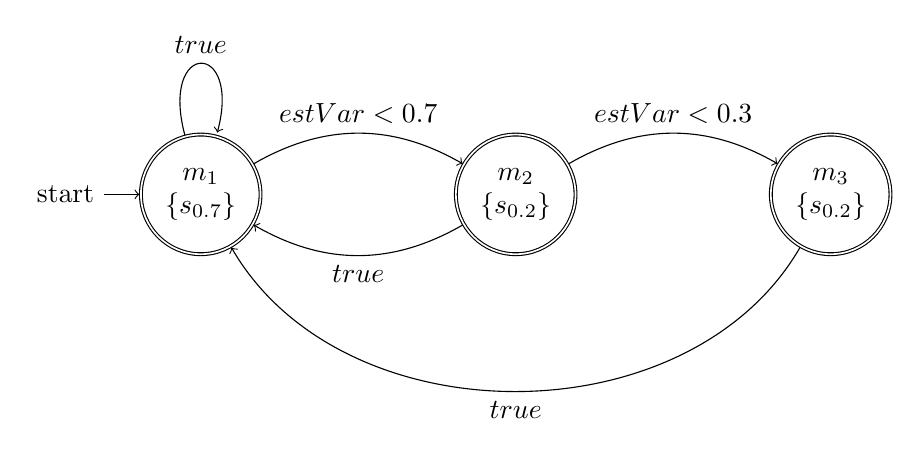
\begin{tikzpicture}[node distance=4cm, text centered, auto]
    \node (A) [state, accepting, text width=1cm, initial] {$m_1$ $\{s_{0.7}\}$};
    \node (B) [state, accepting, text width=1cm] [right of=A] {$m_2$ $\{s_{0.2}\}$};
    \node (C) [state, accepting, text width=1cm] [right of=B] {$m_3$ $\{s_{0.2}\}$};
    
    \path[->] (A) edge [loop above] node {$true$} (A);
    %\path[->] (A) edge [bend left] node {$\neg est_{bad} \wedge s_{0.2}$} (B);
    \path[->] (A) edge [bend left] node {$estVar < 0.7$} (B);
    \path[->] (B) edge [bend left] node {$true$} (A);
    %\path[->] (B) edge [loop above] node {$\neg var3$} (B);
    %\path[->] (B) edge [bend left] node {$est_{good} \wedge s_{0.2}$} (C);
    \path[->] (B) edge [bend left] node {$ estVar < 0.3$} (C);
    %\path[->] (C) edge [loop above] node {$var1$} (C);
    \path[->] (C) edge [bend left=60] node {$true$} (A);
    
    
    \end{tikzpicture}
    
    \caption{Example of guarded automata for our vision based sensor task, in this example the task has two operation modes, $\mathbf{s_{0.7}}$ which need 70\% of the time slot but is more accurate vision computation and $\mathbf{s_{0.2}}$ which is less accurate but faster (need only 20\% of the slot).
        The value of $estVar$ is $var(x-\tilde{x})$ of the previous iteration.
        Every time slot exactly one of the modes will be executed.
        \label{fig:sched_sense_auto}}
\end{figure}

\begin{figure}[]
    \centering
    
    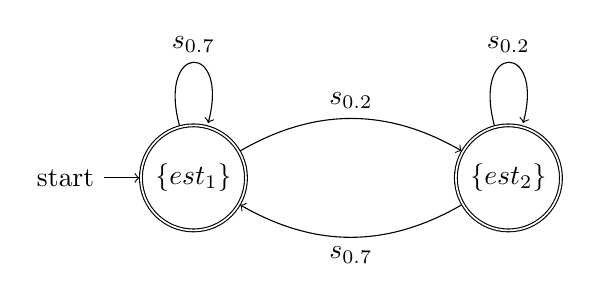
\begin{tikzpicture}[node distance=4cm,auto]
    \node (A) [state, accepting, initial] {$\{est_1\}$};
    \node (B) [state, accepting] [right of=A] {$\{est_2\}$};
    
    \path[->] (A) edge [loop above] node {$s_{0.7}$} (A);
    \path[->] (B) edge [bend left] node {$s_{0.7}$} (A);
    %\path[->] (A) edge [bend left] node {$s_{0.2} \wedge est_2$} (B);
    %\path[->] (B) edge [loop above] node {$s_{0.2} \wedge est_2$} (B);
    \path[->] (A) edge [bend left] node {$s_{0.2}$} (B);
    \path[->] (B) edge [loop above] node {$s_{0.2}$} (B);
    %\path[->] (B) edge [bend left] node {$s_{0.7} \wedge est_1$} (A);
    
    \end{tikzpicture}
    
    \caption{Example of guarded automata for our state estimator, in this example the estimator has two operation modes, $\mathbf{est_1}$ correspond to $\mathbf{s_{0.7}}$ and $\mathbf{est_2}$ correspond to $\mathbf{s_{0.2}}$~(see Figure \ref{fig:sched_sense_auto}).
        \label{fig:sched_estimator_auto}}
\end{figure}

Let us demonstrate the proposed automata based interface using the system depicted in Figure~\ref{fig:hybrid_loop}.
Assume we have two operation modes of the vision based sensor: (1) $s_{0.7}$ a very accurate operation mode that takes 70\% of the time slot to execute, that is of course a significant amount of time, and (2) $s_{0.2}$ a less accurate operation mode but takes only 20\% of the slot.
In each time slot we can execute one of them and get the sensing process done, but if we use only $s_{0.7}$ every time slot we may not have enough time to execute all the tasks. On the other hand, if we use only $s_{0.2}$ we will have inferior estimates.
Figure~\ref{fig:sched_sense_auto} shows an example of a guarded automata that guides the schedule. With this automata we can express rich specifications. 
In this example, execute $s_{0.7}$ is always allowed but if we need faster sensing we can use $s_{0.2}$ but only once in a row if the estimation error is not extremely bad~(if~$var(x-\tilde{x}) < 0.7$), or even twice in a row if the estimation error is good~(if~$var(x-\tilde{x}) < 0.3$).

The estimated estimation error ($estVar$ in the figure) is, in this case, the estimation error variance ($var(x-\tilde{x})$ in Figure~\ref{fig:hybrid_loop}). 
%if $var(x-\tilde{x})$ is small then $est_{good} = true$, if is normal then $est_{normal} = true$ end $est_{bad} = true$ if $var(x-\tilde{x})$ is  bigger then some boundary.
\\This value ($estVar~=~var(x~-~\tilde{x})$) is calculated by the state estimator task (Section~\ref{sec:estimator}) and is passed to the scheduler as discussed before.

Each of this operation modes ($s_{0.7}$ and $s_{0.2}$) have different accuracy, specified by $var(v)$ in Figure~\ref{fig:hybrid_loop}, and if we want to get optimal estimation the state estimator mast be configure correspondingly, i.e., the sensing error variance should be adjusted to the correct value ($var(s_{0.7})$), an easy solution for specifying the different configurations is by the guarded automata shown in Figure~\ref{fig:sched_estimator_auto}, which defines two operation modes of the state estimator, $est_1$ and $est_2$, that correspond to $var(s_{0.7})$ and $var(s_{0.2})$. So of course if we sense in mode $s_{0.7}$ we must estimate with mode $est_1$ that has the correct configurations for $s_{0.7}$, and if we sense in mode $s_{0.2}$ we must estimate with mode $est_2$.





\subsubsection{Automata Operation}
% TODO - mybe as apendex 
\subsubsection{GOAL Tool}
% TODO - mybe as apendex 
\subsubsection{Scheduler Prototype}
% TODO - mybe as apendex 




\section{Proof of Concept}
\label{sec:concept}

%explain that we developing an idea that culd in the future become a tool

\subsection{Simulations}
% TODO - this part is a litle bil lie
% show some matlab simulations of hybrid systems, that have beter resoults with variable time slots

\subsection{Experiment: Vision based controllers for drones}
% overview of why we use vision example
To test our concepts, we will examine the implementation of an autonomously flying quad-rotor in the context of an agriculture case study. Specifically, we will implement a quad-rotor that flies in corridors and greenhouses by a vision based feedback. The challenge in this case study, from our perspective, is that image processing is a heavy computational task that requires careful scheduling in order to preserve the system predictability and stability.

The current state-of-the-art solution for involving heavy computational tasks such as vision in the control system is simply by adding computational power to the system (use faster processors), usually much more than needed, in order to eliminate the chance of loosing predictability.
Some, more conservative, control engineers prefers to isolate the heavy computation from the core control loop by allocating one of the processor's core for that task, or even run the vision processing on a different computer (APM, for example suggests to use image processing by adding a dedicated computer board~\cite{APM}).

In Section~\ref{sec:Research Plan} we propose an alternative framework for such systems, to be implement in the proposed thesis, that allows to integrate the heavy computations in the control loop in an efficient way that, we believe, will allow fo cutting the costs involved in adding a dedicated boards or in dedicating a computation core.


%TODO - fix it
\subsubsection{Sensors}
\label{sec:sensors}
%Anitime reserch of zilbershtain (\cite{Shlomo})
%contract based
%http://ardupilot.org/copter/docs/common-mouse-based-optical-flow-sensor-adns3080.html

\textit{Computer~Vision~Based~Sensor} is the module that is responsible for taking a picture or a series of pictures and produce measurements of quantities such as speed and position relative to the environment.
In our research we will use the \textit{Computer~Vision} in order to detect two dimensional movement in the camera surface (i.e., the drone speed).
There are many such algorithms (called optical flow) differing in running times and in accuracy. Usually more invested time leads to more accuracy.

In our case we need to be able to control the \textit{Computer~Vision} running time and to have some good knowledge of the solution accuracy in order to achieve optimal state estimation (see Section~\ref{sec:estimator}).
We assume that the \textit{Computer~Vision} error is distributed normally, and we will use the error variance as a measure of accuracy. 
We believe that this is a reasonable assumption because the estimated speed is usually computed as the avarage of of many independent random variables, as follows. Optic flow algorithms usually go by identifying similar regions in consecutive pictures and then averaging the distances that each feature ``traveled''. Assuming that the error in measurement of each feature is independent of the other errors, we get that the total error is the average of independent random variables. Then, by the law of large numbers, we get that the error should have a normal distribution. We will validate this assumption by experimentation with different parameters of different algorithms.

%TODO - reed a litle the article (\cite{UPenn-Pant}) and re-write the next.
%TODO - check if Anitime reserch (\cite{Shlomo}) can fit here.
%TODO - Make sure that we use the terms contract-base and any-time correctly
In order to control the running time, we will use anytime based algorithms~\cite{Shlomo} and will mainly concentrate on ``contract based" vision algorithms proposed by Pant~\cite{UPenn-Pant}.
This type of algorithms run until we stop them, and when we stop them they will provide a solution with accuracy that is a monotonic function of the amount of time it was running. That way we can control the solution accuracy by controlling the running time.
In our implementation, in order to lower the complexity, we will pre-define few specific ``operation modes" of the \textit{Computer~Vision} task, that differ by their running time and they are identified by a pair $\langle RunTime, Variance \rangle$ where $Variance$ is the error variance of running time $RunTime$.



\comment{
\subsection{Nano-Satellite}
Another case study we will examine is the control of a nano-satellite. Specifically, we will examine how our new approach can be applied in the context of scheduling the sensing tasks of IAI (Israel Aerospace Industries) nano satellites. Their satellites are controlled by a small, relatively slow, processor and the developers say that a central issue in programing the satellite is how to schedule sensing tasks.
The current approach they are using is to periodically schedule all the sensing task every iteration, and they say that, because of sensor redundancy, this is the main computational consumption and is becoming to be too much for the capabilities of their processor.

We think that much of the sensing is unnecessary and that the controlling task can be achieved without ``most up-to-date" information. Some times we can base on good estimation of the sensing value or even use the last value. As a secondary goal to our main goal of designing a good architecture for vision based drones (our main case study), we will also check the possibility to improve the nano-satellite issue with our framework.
}


\section{Testing Environment}
\label{sec:tests}
\subsection{APM Controlled Quad-copter}
\subsection{Vision based Autonomous In-Door Flying}

%Anitime reserch of zilbershtain (\cite{Shlomo})
%contract based
%http://ardupilot.org/copter/docs/common-mouse-based-optical-flow-sensor-adns3080.html

\textit{Computer~Vision~Based~Sensor} is the module that is responsible for taking a picture or a series of pictures and produce measurements of quantities such as speed and position relative to the environment.
In our research we will use the \textit{Computer~Vision} in order to detect two dimensional movement in the camera surface (i.e., the drone speed).
There are many such algorithms (called optical flow) differing in running times and in accuracy. Usually more invested time leads to more accuracy.

In our case we need to be able to control the \textit{Computer~Vision} running time and to have some good knowledge of the solution accuracy in order to achieve optimal state estimation (see Section~\ref{sec:estimator}).
We assume that the \textit{Computer~Vision} error is distributed normally, and we will use the error variance as a measure of accuracy. 
We believe that this is a reasonable assumption because the estimated speed is usually computed as the avarage of of many independent random variables, as follows. Optic flow algorithms usually go by identifying similar regions in consecutive pictures and then averaging the distances that each feature ``traveled''. Assuming that the error in measurement of each feature is independent of the other errors, we get that the total error is the average of independent random variables. Then, by the law of large numbers, we get that the error should have a normal distribution. We will validate this assumption by experimentation with different parameters of different algorithms.

%TODO - reed a litle the article (\cite{UPenn-Pant}) and re-write the next.
%TODO - check if Anitime reserch (\cite{Shlomo}) can fit here.
%TODO - Make sure that we use the terms contract-base and any-time correctly
In order to control the running time, we will use anytime based algorithms~\cite{Shlomo} and will mainly concentrate on ``contract based" vision algorithms proposed by Pant~\cite{UPenn-Pant}.
This type of algorithms run until we stop them, and when we stop them they will provide a solution with accuracy that is a monotonic function of the amount of time it was running. That way we can control the solution accuracy by controlling the running time.
In our implementation, in order to lower the complexity, we will pre-define few specific ``operation modes" of the \textit{Computer~Vision} task, that differ by their running time and they are identified by a pair $\langle RunTime, Variance \rangle$ where $Variance$ is the error variance of running time $RunTime$.
\subsection{Reference Measurement: Optitrack system}
\subsection{Test Results}


\section{Conclusions and Future Work}
% use real vision
% develop the framwork
% invent mathematical / aupomatic technics to create the automata

\section{Apendix}
\subsection{Kalman Filter and State Estimation}
\label{sec:kalman}
Te role of state estimation as the name suggest is to estimate the current state of the system, usually represented as the vector $x$.
One can monitor the system with an array of sensors, the measurement devices intend to be uncertain, the measurement vector noted by $y=Cx+v$ where $v$ represent the measurement error.
Another estimation technique would be prediction, the system dynamics are known and the system inputs ($u$) are known, then create a model of the system using physics equations to predict the system state evolution in time (assume the initial state is known).
The predicted state, noted by $\hat{x}$, is also not precise the real world is too complex to express in reasonable way, and we mark the predicted error by $w$.

In order to improve the estimation certainty a \textit{filter} is added to the state estimation process, the filter aggregate the sensors and produce better estimation of the state.
We will cover two well known filters, \textit{complementary filter} and \textit{Kalman filter}.

A short brief on \textit{complementary filter}, this is basically combination of two filters (witch are complement each other), in control field it usually refers to \textit{Low-Pass filter} and \textit{High-Pass filter}.
Low-pass filter allows the low frequencies signals to pass and filter out the high frequencies signals, is used for signals with high frequency error, e.g accelerometer signal.
high-pass filter is its complementary, meaning it filters out the low frequencies signals, is used for signals like gyroscope that have continuous accumulated error.
%TODO - more acurate the usage of the signals is expose to high / low errors
\\General complementary filter notation: $\hat{f} = \alpha \cdot f_h + (1-\alpha) \cdot f_l$ s.t. $\alpha \in [0,1]$
%TODO - this is formula for time steping calculation, and this is not realy 
\\if $\alpha$ is significant high, $f_l$ is considered \textit{low-pass}, as rapid value changes less significant and d slow value changes can be accumulated over time, and $f_h$ is considered \textit{high-pass}.
In vision base measurements we use the only Low-pass filter:
$ \hat{x}_k = \hat{x}_{k-1} + \alpha \cdot (y_k - \hat{x}_{k-1}) $.

%TODO - in what sens is optimal?
Complementary and Low-pass are simple and very easy to implement but they not necessary produce the best possible estimation.
A well known estimator called \textit{Kalman filter} is a more complex but optimal filter, Kalman filter assume linear system ($x_{k}=Ax_{k-1} + Bu_{k} + w_{k}$) and zero mean Gaussian errors with covariance matrices $cov(w_k)=Q$ and $cov(v_k)=R$, if those conditions holds kalman filter produce the best possible estimation, based on all previous information available.

This is recursive algorithm that works in a two-step process, \textit{prediction} step and \textit{update} step. 
In the prediction step, the system model used to predict the current state, this called \textit{A Priory Estimate} and noted by $\hat{x}_k^-$,
the error covariance $P_k^-$ of the prediction is also calculated.
Then in the \textit{update} step the prediction is updated to find out the optimal estimation called \textit{A Posteriori Estimate} noted by $\hat{x}_k$) and it's error covariance $P_k$.
Practically the update step is a weighted average between the prediction ($P_k^-$) and the measurement ($y_k$), with more weight being given to estimates with higher certainty~\cite{Kalman-filter}. 

assumes the true state at time $k$ is evolved from the state at $(k − 1)$ according to:
$$x_{k}=Ax_{k-1} + Bu_{k} + w_{k}$$
and the measurement at time $K$ is:
$$y_k=Cx_k+v_k$$
Where $x_k$ is the system state at time step $k$ and $y_k$ is the measurement by the sensors at time step $k$.
%TODO - here we use covariance matrix couse the state variables may be dependent
$w_k$ and $v_k$ represent the process and measurement noise with covariance matrices $Q$ and $R$.
The system state at time $k-1$ ($x_{k-1}$) is unknown, therefore the previous estimation is used to predict the next step state using the recursive equation:
$$ \hat{x}_{k}^-=A\hat{x}_{k-1} + Bu_{k} $$
the error covariance of the prediction composed of the error of previous estimation which is:
$cov(A\hat{x}_{k-1} - x_{k-1}) = A cov(\hat{x}_{k-1} - x_{k-1}) A^T=A P_{k-1} A^T$
and the process error of time $k$ ($Q$) and we get prediction error covariance of:
$$ P_k^- = A P_{k-1} A^T + Q $$

After the prediction was calculated the update step combine the prediction and measurements to get the Kalman estimation:
$$ \hat{x}_{k} = \hat{x}_{k}^- + K_k(y_k - C\hat{x}_{k}^-)$$
$K_k$, also called Kalman Gain, represent contribution each partial estimation ($\hat{x}_{k}^-$ and $y_k$) to the Kalman estimation, and is calculate each time by:
$$ K_k = {{P_k^- C^T} \over {C P_k^- C^T + R} }$$
And the Kalman estimation covariance is:
$$ P_k = (I - K_kC) P_k^- $$

The Kalman filter is designed for linear systems. It is not suitable in the case of a nonlinear systems, if the state transition function or the measurement function are nonlinear:
$$x_{k}=f(x_{k-1} , u_{k}) + w_{k}$$
$$y_k=h(x_k) + v_k$$
A Kalman filter that linearizes the nonlinear function around the mean of current state estimation is used, this referred to as an extended Kalman filter (EKF).
The transition and mesurment functions must be differentiable in order to linearize them, and the Jacobian matrices are used.
Extended Kalman filter is not guaranty to be optimal filter.

%TODO - there is "Uncertail KF" that improve the linearity estimation in extream cases (not realy understand it) but could be good example of high computational consumption of well known estimator


%TODO - think this need to be in the architecture section
\comment{
In order to produce optimal estimation with Kalman filter, one of the parameter that we need to consider in our calculation is the variance of the sensor error.
But in our new framework the sensor (vision based sensor) have variable error variance for each time slot, this means that we need to have also variable state estimators correspondingly.
In order to adjust the sensor error variance, each time step the scheduler will inform the state estimator about the new error variance, and the state estimator will use corresponding parameters to make the next estimation.

APM, the control software that we will use, is already using kalman filter as the state estimator, so we only need to adjust the existing module to the variable sensor error variance, and to send the estimation error variance to the scheduler (see Section~\ref{sec:scheduler}).
}

\subsection{TODO}


\comment{
\section{Research Plan}
\label{sec:Research Plan}
Our research plan consists of: (1) Designing a methodology for effective allocation of computational resources in real-time control systems; and then (2) Demonstrating our methodology with a framework for developing such systems and with a case study. The details of these two steps are elaborated below.




\subsection{The proposed methodology}
\label{sec:our proposal}
%TODO - re-write, probably need to be renamed to arcitecture

The general methodology that we will develop is illustrated in Figure~\ref{fig:general_hybrid_loop}.
The methodology comes to support an efficient scheduling protocols in modern control systems consisting of a computer that runs many tasks that implement the control laws of independent control loops. 
The current state of art, as describrd above and we observed, e.g., in the code of the APM~\cite{APM}, is that the designers of each control loop specify a fixed rate for invocations of the corresponding control task.
%That methodology is based on modern controller architecture where the system has multiple controlling tasks (control loops) and a scheduler that schedule the task as they demand.
% TODO: Use the terminology of the figure
In our methodology, shown in Figure~\ref{fig:general_hybrid_loop}, there is a richer interaction between the \textit{Scheduler} and the control loops. We suggest that each control loop (blue components) will tell the resource allocator (\textit{scheduler}) of its level of certainty and that the allocator will base its allocation of CPU time based on this data. This can be useful on its own sake or together with a mathematical analysis that allows to use this feedback mechanism to certify some pre-defined specifications of state certainty or stability is maintained.

Our proposed methodology is general and may be applicable in a wide range of applications. However, in this initial phase of the research, we believe that it is better to focus on a specific sub-domain and in handling all technical issues in order to prove the concept.
In this thesis we will develop and implement the, more specific, framework shown in Figure~\ref{fig:hybrid_loop}: a vision based controller for drone. 

As shown in Figure~\ref{fig:hybrid_loop}, the suggested control system framework consists of an interaction between the tasks scheduler and the control loops, in this case the estimation task (\textit{State~Estimation}) accuracy strongly depends on the sensing task (\textit{Computer~Vision}) and they both collaborate with the \textit{scheduler} in order to achieve their \textbf{control objectives} (g.e. stability).
In this framework the scheduler is part of the control logic and therefore it can make scheduling decisions based on the current control state, the scheduling of \textit{Computer~Vision} task depends on the accuracy of state estimation.
For example, if the vision is clear, the \textit{Computer~Vision} will produce good measurement of the \textit{System} and therefore good accuracy will be achieved so the \textit{Scheduler} can allocate less computation time to the heavy \textit{Computer~Vision} task and still remain stable while allocating more CPU to others control loops or to background tasks (like navigation).

We will use an existing open-source implementation of drone software as a basis for our experimentation. However, the above collaboration requires to re-adjust some parts of the control system, e.g. the \textit{State~Estimator} needs to work with variable error variance of \textit{Computer~Vision} measurement,  the \textit{Computer~Vision} needs to be able run within variable time limits, and the tasks pre-defined requirements need to be re-adjusted in order to define the relation between tasks such as \textit{Computer~Vision} and \textit{State~Estimator}.
Below we will dive in each part of the above system (Figure~\ref{fig:hybrid_loop}) and explain how it will be adjusted (changed) and how we will achieve that adjustment in our demonstration.

%Finally, we need to re-consider the system Analyzing technique because variable sensing characteristics (\textit{Computer~Vision} time limits) will lead to variable estimation characteristics... %TODO - complete and fix this paragraph or remove it

\subsubsection{Sensors (\textit{Computer~Vision~Based~Sensor})}
\label{sec:sensors}
%Anitime reserch of zilbershtain (\cite{Shlomo})
%contract based
%http://ardupilot.org/copter/docs/common-mouse-based-optical-flow-sensor-adns3080.html

\textit{Computer~Vision~Based~Sensor} is the module that is responsible for taking a picture or a series of pictures and produce measurements of quantities such as speed and position relative to the environment.
In our research we will use the \textit{Computer~Vision} in order to detect two dimensional movement in the camera surface (i.e., the drone speed).
There are many such algorithms (called optical flow) differing in running times and in accuracy. Usually more invested time leads to more accuracy.

In our case we need to be able to control the \textit{Computer~Vision} running time and to have some good knowledge of the solution accuracy in order to achieve optimal state estimation (see Section~\ref{sec:estimator}).
We assume that the \textit{Computer~Vision} error is distributed normally, and we will use the error variance as a measure of accuracy. 
We believe that this is a reasonable assumption because the estimated speed is usually computed as the avarage of of many independent random variables, as follows. Optic flow algorithms usually go by identifying similar regions in consecutive pictures and then averaging the distances that each feature ``traveled''. Assuming that the error in measurement of each feature is independent of the other errors, we get that the total error is the average of independent random variables. Then, by the law of large numbers, we get that the error should have a normal distribution. We will validate this assumption by experimentation with different parameters of different algorithms.

%TODO - reed a litle the article (\cite{UPenn-Pant}) and re-write the next.
%TODO - check if Anitime reserch (\cite{Shlomo}) can fit here.
%TODO - Make sure that we use the terms contract-base and any-time correctly
In order to control the running time, we will use anytime based algorithms~\cite{Shlomo} and will mainly concentrate on ``contract based" vision algorithms proposed by Pant~\cite{UPenn-Pant}.
This type of algorithms run until we stop them, and when we stop them they will provide a solution with accuracy that is a monotonic function of the amount of time it was running. That way we can control the solution accuracy by controlling the running time.
In our implementation, in order to lower the complexity, we will pre-define few specific ``operation modes" of the \textit{Computer~Vision} task, that differ by their running time and they are identified by a pair $\langle RunTime, Variance \rangle$ where $Variance$ is the error variance of running time $RunTime$.

\subsubsection{State Estimator}
\label{sec:estimator}
% kalman filter & ...
% seperation rule of kalman

In cases where we have uncertain observations (inaccurate sensors), e.g. the computer vision measurement, we prefer to make some \textbf{educated estimation} of the current state based on the uncertain observations rather than just consider the last observation as the current state.
This \textbf{educated estimation} of the current state is the main goal of the \textit{State~Estimator} block.
This block receives the raw data from the sensors and produce an estimation of the current state.

In this thesis we will use well known optimal estimator called Kalman filter, or, more generally, extended Kalman filter (EKF) which is the nonlinear version of Kalman filter.
The algorithm works in a two-step process. In the prediction step, the Kalman filter produces estimates of the current state variables, along with their uncertainties. Once the outcome of the next measurement is observed, these estimates are updated using a weighted average, with more weight being given to estimates with higher certainty~\cite{Kalman-filter}. 

In order to produce optimal estimation with Kalman filter, one of the parameter that we need to consider in our calculation is the variance of the sensor error.
But in our new framework the sensor (vision based sensor) have variable error variance for each time slot, this means that we need to have also variable state estimators correspondingly.
In order to adjust the sensor error variance, each time step the scheduler will inform the state estimator about the new error variance, and the state estimator will use corresponding parameters to make the next estimation.

APM, the control software that we will use, is already using kalman filter as the state estimator, so we only need to adjust the existing module to the variable sensor error variance, and to send the estimation error variance to the scheduler (see Section~\ref{sec:scheduler}).

\subsubsection{Control Tasks} 
\label{sec:control}
The control task itself (\textit{Control Law} in Figure~\ref{fig:general_hybrid_loop}) is responsible for reducing the difference between the current state ($x$) where $\tilde{x} = x+ ``estimation~error"$ (in Figure~\ref{fig:general_hybrid_loop}) and the target state ($u$ in Figure~\ref{fig:general_hybrid_loop}), by manipulating the drone motors speed.

%Optimal estimation or optimal control low is not guarantee the overall  optimal feedback controller, but as Kalman prove, 
The control task is usually a very low CPU consumer and been well studied~\cite{Bennett,Cervin}. Hence, in the proposed thesis, we will not focus on the control task and will use the existing controller that APM are using.
APM use a commonly used and well known technique from control theory called PID, A proportional-integral-derivative controller.
In this technique the control output is based on the physical knowledge of the system dynamics, and have three variable parameters (P, I and D) that define the controller convergence behavior.

We also plan to try to use an ``adjustable'' LQR (Linear-quadratic regulator) control, as follows.
LQR is an optimal controller that take into account the level of certainty of the state estimation. 
Is usually a hard task to know the certainty of estimation, but in our case we need to calculate it anyway, and we mark it as $var(x-\tilde{x})$.
We will make LQR ``adjustable'' in the sense that each iteration the controller will consider the new (variable) $var(x-\tilde{x})$. This is similar to the architecture we proposed for the estimator.
We will check if adjustable LQR has significant advantages over PID in cases were we have variable certainty of estimation.

\subsubsection{Computation Resource Scheduler: Automata Based Scheduler}
\label{sec:scheduler}

Real-time systems are mostly composed of multiple real-time tasks, tasks with time constraint, for example task that must response within specified time constraints.
The purpose of schedulers in such systems is to allocate the limited computational resources (CPU time) within all the task in the system. To do so, we need a well defined interface between the real-time tasks and the scheduler.

The most common way of describing the requirements of a real-time component is to specify a period, sometimes along with a deadline, which gives the frequency at which the component must execute. The designer of the component makes sure that the performance objectives are met as long as the component is executed consistent with its period. The scheduler guarantees that all components get enough resources.
%not directly in this article
Specifying resource requirements using periods has advantages due to simplicity and analyzability, but has limited expressiveness, as elaborated in~\cite{RTComposer}. 
%For example, a specification such as “execute the component every 5ms” does not say whether the scheduler should or should not execute it more frequently if enough computing resources are available, and if a component has multiple methods, say, for different control tasks, each needing a different period, the requirement cannot be naturally captured by a single period.

In this thesis one of the main goals, as we said above in Section~\ref{sec:Research Plan}, is to develop a methodology for allocation resources. We will focus on proposing way for engineers to describe the requirements of a real-time component.
To simplify, we will assume that the resource is allocated in discrete slots of some fixed duration in the style of time-triggered architecture~\cite{RTComposer}.
We will develop automata based (hybrid automata) methodologies and schedulers based on the work of Alur~\cite{RTComposer} and Bukra~\cite{Merav}, and will demonstrate with measurable data how they improve the performance of real flying drones (see Section~\ref{sec:results}).
%We will use finite automata over infinite words as specification framework for resource requirements, automata can be more expressive, for describe more specific requirements, and they are composable, it is easy to compose all the tasks requirements into one automata. 

We will use hybrid automata as specification framework for resource requirements.
Hybrid automata is a variation of finite automata for real-valued continuously progressing words~\cite{hibrid-systems}.
Automata can be more expressive for describing specific requirements, and they are composable, i.e., it is easy to compose all the tasks requirements into an integrated automaton.
In our setting, the hybrid automata define continuous (fixed period) operation modes, represented by the automata state, and the condition of mode changing (mode transition) are denoted by the edges in the automata.
The operation mode directly define a set of tasks that will be executed in the time slot (for example $s_{0.7}$ in Figure~\ref{fig:sched_sense_auto}).
We can stay at a single mode for some iterations, in this case the same tasks will be scheduled in each iteration. 
We can also take \textbf{discrete mode transition} in order to change operation mode after few iterations and schedule different set of tasks, for example, in Figure~\ref{fig:sched_sense_auto} the edge $(m_1,m_2)$ says that if the previous iteration mode was $m_1$ and $estVar < 0.7$ we can change the mode and schedule the set $\{s_{0.2}\}$ in the next iteration.

Each infinite path on the composed hybrid automata (not necessarily with infinitely many mode transitions) represents a schedule that satisfy all the tasks requirements. 
In this architecture the scheduler only need to ``walk through'' the composed automata, this is, of course, a fast and easy computational task. 
In order to assure that we do not exceed the time slot duration, each task will have pre-defined maximum duration time like ``deadline'' in the traditional architecture. Now we can verify that every possible scheduling step can execute within a single time slot, in other words, every mode of the composed automata can be executed in a single time slot, by simply summing the ``deadlines'' of all the tasks in the mode tasks set.
%we can summarize the total slot ``deadline'' as follows:\\
%$\forall mode~e ~~(\sum_{t \in Guard(e)} deadline(t) ) \leq slot~duration$ \\
If we find a mode that goes beyond the maximum duration we can remove it from the automata so we never exceed the time slot duration.


\begin{figure}[]
    \centering
    
    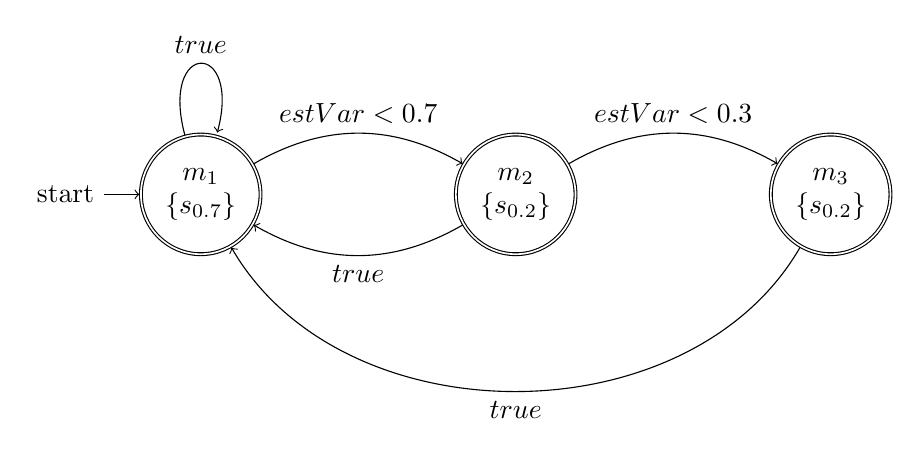
\begin{tikzpicture}[node distance=4cm, text centered, auto]
        \node (A) [state, accepting, text width=1cm, initial] {$m_1$ $\{s_{0.7}\}$};
        \node (B) [state, accepting, text width=1cm] [right of=A] {$m_2$ $\{s_{0.2}\}$};
        \node (C) [state, accepting, text width=1cm] [right of=B] {$m_3$ $\{s_{0.2}\}$};
        
        \path[->] (A) edge [loop above] node {$true$} (A);
        %\path[->] (A) edge [bend left] node {$\neg est_{bad} \wedge s_{0.2}$} (B);
        \path[->] (A) edge [bend left] node {$estVar < 0.7$} (B);
        \path[->] (B) edge [bend left] node {$true$} (A);
        %\path[->] (B) edge [loop above] node {$\neg var3$} (B);
        %\path[->] (B) edge [bend left] node {$est_{good} \wedge s_{0.2}$} (C);
        \path[->] (B) edge [bend left] node {$ estVar < 0.3$} (C);
        %\path[->] (C) edge [loop above] node {$var1$} (C);
        \path[->] (C) edge [bend left=60] node {$true$} (A);
                

    \end{tikzpicture}
    
    \caption{Example of guarded automata for our vision based sensor task, in this example the task has two operation modes, $\mathbf{s_{0.7}}$ which need 70\% of the time slot but is more accurate vision computation and $\mathbf{s_{0.2}}$ which is less accurate but faster (need only 20\% of the slot).
    The value of $estVar$ is $var(x-\tilde{x})$ of the previous iteration.
    Every time slot exactly one of the modes will be executed.
    \label{fig:sched_sense_auto}}
\end{figure}

\begin{figure}[]
    \centering
    
    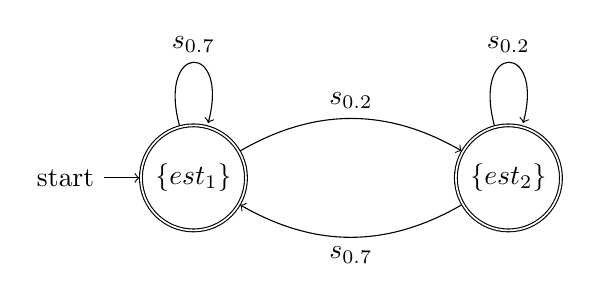
\begin{tikzpicture}[node distance=4cm,auto]
        \node (A) [state, accepting, initial] {$\{est_1\}$};
        \node (B) [state, accepting] [right of=A] {$\{est_2\}$};
        
        \path[->] (A) edge [loop above] node {$s_{0.7}$} (A);
        \path[->] (B) edge [bend left] node {$s_{0.7}$} (A);
        %\path[->] (A) edge [bend left] node {$s_{0.2} \wedge est_2$} (B);
        %\path[->] (B) edge [loop above] node {$s_{0.2} \wedge est_2$} (B);
        \path[->] (A) edge [bend left] node {$s_{0.2}$} (B);
        \path[->] (B) edge [loop above] node {$s_{0.2}$} (B);
        %\path[->] (B) edge [bend left] node {$s_{0.7} \wedge est_1$} (A);

    \end{tikzpicture}
    
    \caption{Example of guarded automata for our state estimator, in this example the estimator has two operation modes, $\mathbf{est_1}$ correspond to $\mathbf{s_{0.7}}$ and $\mathbf{est_2}$ correspond to $\mathbf{s_{0.2}}$~(see Figure \ref{fig:sched_sense_auto}).
    \label{fig:sched_estimator_auto}}
\end{figure}

Let us demonstrate the proposed automata based interface using the system depicted in Figure~\ref{fig:hybrid_loop}.
Assume we have two operation modes of the vision based sensor: (1) $s_{0.7}$ a very accurate operation mode that takes 70\% of the time slot to execute, that is of course a significant amount of time, and (2) $s_{0.2}$ a less accurate operation mode but takes only 20\% of the slot.
In each time slot we can execute one of them and get the sensing process done, but if we use only $s_{0.7}$ every time slot we may not have enough time to execute all the tasks. On the other hand, if we use only $s_{0.2}$ we will have inferior estimates.
Figure~\ref{fig:sched_sense_auto} shows an example of a guarded automata that guides the schedule. With this automata we can express rich specifications. 
In this example, execute $s_{0.7}$ is always allowed but if we need faster sensing we can use $s_{0.2}$ but only once in a row if the estimation error is not extremely bad~(if~$var(x-\tilde{x}) < 0.7$), or even twice in a row if the estimation error is good~(if~$var(x-\tilde{x}) < 0.3$).

The estimated estimation error ($estVar$ in the figure) is, in this case, the estimation error variance ($var(x-\tilde{x})$ in Figure~\ref{fig:hybrid_loop}). 
%if $var(x-\tilde{x})$ is small then $est_{good} = true$, if is normal then $est_{normal} = true$ end $est_{bad} = true$ if $var(x-\tilde{x})$ is  bigger then some boundary.
\\This value ($estVar~=~var(x~-~\tilde{x})$) is calculated by the state estimator task (Section~\ref{sec:estimator}) and is passed to the scheduler as discussed before.

Each of this operation modes ($s_{0.7}$ and $s_{0.2}$) have different accuracy, specified by $var(v)$ in Figure~\ref{fig:hybrid_loop}, and if we want to get optimal estimation the state estimator mast be configure correspondingly, i.e., the sensing error variance should be adjusted to the correct value ($var(s_{0.7})$), an easy solution for specifying the different configurations is by the guarded automata shown in Figure~\ref{fig:sched_estimator_auto}, which defines two operation modes of the state estimator, $est_1$ and $est_2$, that correspond to $var(s_{0.7})$ and $var(s_{0.2})$. So of course if we sense in mode $s_{0.7}$ we must estimate with mode $est_1$ that has the correct configurations for $s_{0.7}$, and if we sense in mode $s_{0.2}$ we must estimate with mode $est_2$.

\section{Preliminary Work and Results}
\label{sec:results}
In this preliminary phase we searched for the appropriate environment for experimentation. After research we decided to use Raspberry~Pi with the navio~\cite{navio} board based drone with the commonly used and open-source controller software APM~\cite{APM}.
We managed to build and fly the complete drone, we dived into the APM code, we understand the code structure, and we are familiar with the relevant parts that we want to change.

We now have a clear picture of our research plan for the near future in order to get basic results with the new scheduling framework.
In summary, our research plan is describe in Table~\ref{tab:Research-plan}.

\begin{table}[]
    \centering
    \label{tab:Research-plan}
    
    \begin{tabular}{ | p{8cm} | p{1.7cm} | p{1.8cm} |}
        \hline
        Task  & Expected work time & completion (\%) \\ \hline
        Choose the appropriate development environment. (APM based drones) & one month & \textbf{100\%}  \\ \hline
         
        Be familiar with the development environment, and make sure that we are able to adapt the system to our needs. & three month & \textbf{90\%} \\ \hline
          
        Plan all the control components in order to achieve our case study goals. (see Sections~\ref{sec:estimator}, \ref{sec:sensors} and \ref{sec:control}) & three months & \textbf{100\%} \\ \hline
         
        Plan the new scheduler detail behavior, and it’s interaction with the control components. (see Section~\ref{sec:scheduler}) & two months & \textbf{90\%} \\ \hline
         
        Detail planing of the scheduler interface implementation and adaptation in the code. & one month & \textbf{80\%} \\ \hline
         
        Implement the new scheduler and replace the original APM scheduler (manually transform each task periodical requirements to automata based requirements). & two weeks & 0\% \\ \hline
         
        Develop and implement the vision based sensor component. We plan to base on the buit-in Matlab vision abilities and use SimuCopter~\cite{SimuCopter}
        to integrate it in the APM program. & 1-2 months. & 20\% \\ \hline
         
        Grub statistics data and fine-tuning the vision component. & one month & 0\% \\ \hline
         
        Adjust the state estimator as explain in Section~\ref{sec:estimator}, and combine all together using the new scheduler. & two weeks & 0\% \\ \hline
         
        Check with a wide range of environmental conditions and a wide range of requirements (automatas), and of course grub and summarize the results. & two months & 0\% \\ \hline
        
        Write the thesis report. & two months & 10\% \\ \hline
    \end{tabular}
    
    \caption{Research plan}
\end{table}

As part of the preliminary work we developed (with two undergraduate students, as part of their final project in software engineering) the \textbf{SimuCopter}~\cite{SimuCopter} framework that allows to program our drone  (or any other APM based drones) directly by Matlab Simulink model, using a code generation logic.
We will add to that framework interfaces and tools for using our new scheduler capabilities embedded in the simulink diagrams, and give the control engineers a complete tool for developing control software. We also experimented with iplementing computer vision algorithms with this tool.

}
%\begin{samepage}
    \bibliographystyle{plain}
    \bibliography{hodai_thesis}{}
%\end{samepage}


\end{document}}